\documentclass[../main.tex]{subfiles}
\graphicspath{{\subfix{../figures/}}}

\begin{document}
\chapter{Literature Review} \label{chap:review}
In this chapter, I briefly describe our controller and how it can be illustrated in a block diagram. Then, I introduce the critical terms of reinforcement learning (RL) before comparing the pros and cons of some typical schemes in recent papers. Finally, I conclude my approach for this thesis.

\section{RL as a Controller} \label{sec:rl_ctrl}
RL is a type of machine learning that learns to make decisions by performing actions in an environment to maximize a cumulative reward. Unlike supervised learning, which learns from a dataset of labeled examples, RL gets its experience from the consequences of prior actions through trial and error, making it well-suited for tasks that require sequential decision-making.
\begin{figure}[htb]
    \centering
    \begin{subfigure}{0.75\textwidth}
        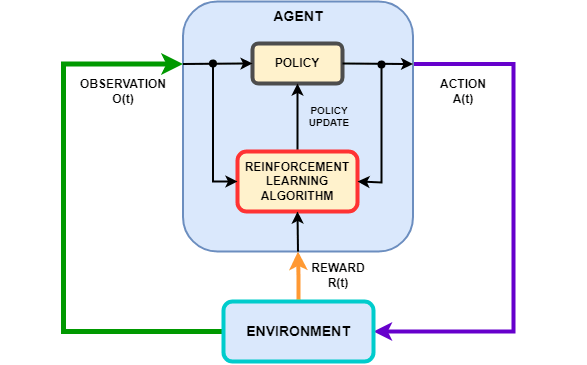
\includegraphics[width=\linewidth]{figures/rl_component.png}
        \caption{Components of RL}
        \label{fig:rl_component}
    \end{subfigure}
    \begin{subfigure}{0.75\textwidth}
        \centering
        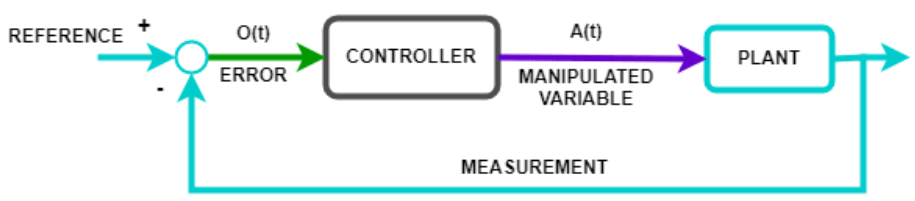
\includegraphics[width=\linewidth]{figures/ctrl_component.png}
        \caption{Components of a control system}
        \label{fig:ctrl_component}
    \end{subfigure}
    \caption{RL as a control system, by MATLAB \cite{MathWorksRLControlSystems}}
    \label{fig:rl_vs_ctrl}
\end{figure}
That is why RL is similar to a control system, as shown in figure \ref{fig:rl_vs_ctrl} made by MATLAB \cite{MathWorksRLControlSystems}, that is:
\begin{itemize}
    \item Policy is a controller; an agent includes both a policy and an algorithm that updates the policy during its learning process.
    \item Environment is the plant with noises, disturbances, filters, sensor feedback, etc.
    \item Observation is the feedback from sensors
    \item Action is the control signal
    \item Reward and learning algorithm are equivalent to the self-adaptation mechanism that exists in modern adaptive controllers
\end{itemize}

A fundamental concept underpinning RL is the Markov Decision Process (MDP), which provides a mathematical framework for modeling decision-making scenarios where outcomes are partially random and under an agent's control. An MDP is defined by a tuple $(\mathbb{S}, \mathbb{A}, P, R, \gamma)$:
\begin{itemize}
    \item \textbf{States $\mathbb{S}$}: a finite or infinite set of all possible states where the agent can exist. State $s \in \mathbb{S}$ represents a situation that the agent witnesses. Thus, some call it an observation vector $\mathbf{o}$ of the observation space $\mathbf{O}$.
    \item \textbf{Actions $\mathbb{A}$}: a finite or infinite set of all possible actions, one of which $a \in \mathbb{A}$ the agent selects based on its state $s$. This action influences both the next state and the reward received.
    \item \textbf{Transition Probability} $P(s^\prime|s, a)$: environment's dynamics that governs the likelihood of transitioning from state $s$ to $s^\prime$ after taking action $a$.
    \item \textbf{Reward Function} $R$: provides immediate feedback $R(s, s^\prime, a)$ after doing $a$ to move from $s$ to $s^\prime$. This signal guides the agent's learning process.
    \item \textbf{Discount Factor} $\gamma$: a value between 0 and 1 that represents the importance of future rewards. A discount factor close to 1 values future rewards similarly to immediate rewards, while a discount factor close to 0 prioritizes immediate rewards.
    \item \textbf{Expected Cumulative Reward} aka. \textbf{discounted future reward G(t)}: the total reward expected to be earned after a sequence of the next $k+1$ steps from time $t$ on.
    \begin{equation}
        \begin{split}
            G_t &= R_{t+1} + \gamma R_{t+2} + \gamma^2 R_{t+3} + \ldots \\
            &= \sum_{k=0}^{\infty} \gamma^{k}R_{t+k+1}
        \end{split}
    \label{eq:future_rwd}
    \end{equation}
\end{itemize}

\textbf{A policy} $\pi: \mathbb{S} \rightarrow \mathbb{A}$ is an agent's behavior that maps states to actions, which can be evaluated by either a \textbf{state value} $V(s)$ (Eq. \ref{eq:vval}) or a \textbf{state-action value} $Q(s, a)$ (Eq. \ref{eq:qval}).
\begin{equation}
    V_{\pi}(s) = \mathbb{E}_{\pi} \left[ \sum_{t=0}^{\infty} \gamma^t R(s_t, a_t, s_{t+1} | s_0 = s) \right]
    \label{eq:vval}
\end{equation}
\begin{equation}
    Q_{\pi}(s,a) = \mathbb{E}_{\pi} \left[ \sum_{t=0}^{\infty} \gamma^t R(s_t, a_t, s_{t+1} | s_0 = s, a_0 = a) \right]
    \label{eq:qval}
\end{equation}
People call them V-value and Q-value functions, respectively. The table \ref{tab:qv_compare} below summarizes when we should choose one over the other as a reward backbone as suggested by Richard S. Sutton\cite{rlbible_mdp}. 
\begin{table}[htb]
    \centering
    \caption{Comparison of V-value and Q-value functions}
    \begin{tabular}{l p{6cm} p{6cm}}
        \toprule
        \textbf{ } & \textbf{V-value} & \textbf{Q-value} \\
        \midrule
        \textbf{Pros} & Simple state evaluation; useful when the policy only compares state quality, i.e., which state is most promising & Direct action evaluation; useful when policy needs to compare actions from a given state \\
        \addlinespace
        \textbf{Cons} & Requires additional steps for action selection; limited use in action selection without additional info & More complex to compute and store in memory, especially for a large action space \\
        \addlinespace
        \textbf{Use when} & Agent only needs to choose which state is the best to transition or when there are infinite actions & Directly deriving an action is necessary; useful with an off-policy agent or when the state-action space is manageable \\
        \bottomrule
    \end{tabular}
\label{tab:qv_compare}
\end{table}
A policy $\pi_1$ is better than another $\pi_2$ if $\pi_1$ eventually returns more reward.
\begin{gather*}
    \pi_1 \geq \pi_2 \\
    \Leftrightarrow
        V_{\pi_1} \geq V_{\pi_2} \lor
        Q_{\pi_1} \geq Q_{\pi_2}
\end{gather*}
A critical property of $V(s)$, $Q(s, a)$, or any other value we might invent in the future is that they must obey the Bellman equation \ref{eq:bellman}.
\begin{equation}
    V_{\pi}(s) = \mathbb{E}_{\pi} \left[G_t | s \right] \text{  , similar for Q-value}
\label{eq:bellman}
\end{equation}

Thus, solving an MDP aims to find an optimal policy $\pi^*$ that maximizes the expected return over time \ref{eq:pistar}, which we will discuss in section \ref{sec:mdp_solutions}.
\begin{equation} \label{eq:pistar}
    \begin{split}
        &\pi^* = \arg\max_{\pi} V_{\pi}(s) \,~ \forall s \in \mathbb{S}\\
        \text{or  }
        &\pi^* = \arg\max_{\pi} Q_{\pi}(s, a) \,~  \forall s \in \mathbb{S},~ a \in \mathbb{A}
    \end{split}
\end{equation}
Reversely, we also say
\begin{equation} \label{eq:vstar}
    \begin{split}
        V^*(s) &= \max_{\pi} V_{\pi}(s) \\
        \text{ or } 
        Q^*(s, a) &= \max_{\pi} Q_{\pi}(s, a)
    \end{split}
\end{equation}

\nomenclature[D]{agent}{A reinforcement learning agent is a controller that interacts with the environment, receives feedback, and learns of past experiences to make better decisions next time.}
\nomenclature[N]{$\mathbb{E}$}{Expected value of a random variable}
\nomenclature[N]{$V(s)$}{State value, aka. V-value denotes the desirability of a state. Standalone notation $V$ means a physical volume of an object}
\nomenclature[N]{$Q(s,a)$}{Action value, aka. Q-value denotes the desirability of an action in a given state.}
\nomenclature[N]{$\pi$}{A policy that maps a state into an action; also known as an actor in the actor-critic framework.}
\nomenclature[N]{$\delta$}{Temporal difference between the reward predicted by a critic and the actual reward given by the environment.}
\nomenclature[N]{$V_{\theta}(s)$, $Q_{\theta}(s,a)$}{Parameterized value functions}
\nomenclature[N]{$\pi_\phi$}{Parameterized policy}
\nomenclature[N]{$\mathbb{S}$}{Observation or state space of a Markov decision process}
\nomenclature[N]{$\mathbb{A}$}{Action space of a Markov decision process.}


\section{Categories of RL Algorithms}
\subsection{MDP Solver} \label{sec:mdp_solutions}
The earliest solution for an MDP is a naive \textbf{dynamic programming (DP)}, invented by Richard E. Bellman \cite{rlbible_mdp} in 1957. In his book, a DP process contains two phases:
\begin{itemize}
    \item \textbf{Value Iteration}: first, it updates the value of each state by considering the expected utility of the possible actions. The update rule is:
    \[
    V_{k+1}(s) = \max_a \sum_{s'} P(s'|s, a) \left[ R(s, a, s') + \gamma V_k(s') \right]
    \]
    where \( V_k(s) \) is the value of state \( s \) at iteration \( k \).
    \item \textbf{Policy Iteration}: then it updates policy via two sub-steps
    \begin{itemize}
        \item \textbf{Policy Evaluation}: compute the value of each state under a fixed policy \( \pi \):
        \[
        V^\pi(s) = \sum_{a} \pi(a|s) \sum_{s'} P(s'|s, a) \left[ R(s, a, s') + \gamma V^\pi(s') \right]
        \]
        \item \textbf{Policy Improvement}: update the policy based on the new value function:
        \[
        \pi'(s) = \arg\max_a \sum_{s'} P(s'|s, a) \left[ R(s, a, s') + \gamma V^\pi(s') \right]
        \]
    \end{itemize}
    \item These steps are alternated until the policy converges to the optimal policy. 
\end{itemize}
Since DP is pure programming, it always finds the same solution given the same input. However, it requires a perfect environment model and is computationally heavy, which is impractical for an infinite state-action space of real-life scenarios.

\textbf{Monte Carlo (MC)} overcomes these two constraints by visiting all states in $S$ to calculate their values $V(s)$ and update its experience via this formula 
\begin{equation}
    V(s) \leftarrow V(s) + \alpha (G_t - V(s))
    \label{eq:montecarlo}
\end{equation}
\begin{itemize}
    \item $\alpha$ is a step size similar to a learning rate in ML.
    \item $\delta_t = G_t - V(s)$ is called an advantage function. This term also works for Q-value, i.e., $\delta_t = G_t - Q(s, a)$
\end{itemize}
 Yet, MC can be slow to converge because it only updates the value estimates at the end of an episode. Nevertheless, an accurate estimate requires many samples.

\textbf{Temporal Difference (TD)} combines the strengths of both DP and MC. It updates value estimates immediately after each step without waiting for an outcome, making it much more efficient. That is why most modern RL algorithms use TD.
\begin{equation} \label{eq:tdv}
    V(s) \leftarrow V(s) + \alpha \left[ r + \gamma V(s') - V(s) \right]
\end{equation}
As noted in table \ref{tab:qv_compare}, the downside of the V-value is that it only depicts how good a situation is, i.e., what maximum reward it possibly earns ahead. Others use Q-value to tell further how good a state is if it takes a specific action.
\begin{equation} \label{eq:tdq}
    Q(s, a) \leftarrow Q(s, a) + \alpha \left[ r + \gamma \max_{a'} Q(s', a') - Q(s, a) \right]
\end{equation}

Table \ref{tab:mdp_solvers} compares these three families of methods to solve a Markov Decision Process problem. In summary, TD is used the most in modern RL, whereas DP and MC only serve for educational purposes.
\begin{table}[htb]
\centering
\caption{Comparison of MDP solving methods}
\begin{tabularx}{\textwidth}{lXXX}
    \toprule
    \textbf{Aspect} & \textbf{DP} & \textbf{MC} & \textbf{TD} \\
    \midrule
    Update Timing & Offline (batch updates) & Offline (episode-based) & Online (incremental updates) \\
    \hline
    Requirement & Requires full MDP knowledge & No need for MDP knowledge & Partial MDP knowledge \\
    \hline
    Stability & Stable if a model is accurate & Stable but can have high variance & Stable with proper tuning \\
    \hline
    Sample Efficiency & Efficient for small state spaces & Requires full episodes & Efficient for online learning \\
    \hline
    Exploration & No exploration (deterministic) & No exploration bias & Balances exploration and exploitation \\
    \hline
    Scalability & Limited to small state-action space & Scales well with data & Scales well with data \\
    \hline
    Bias-Variance & Low variance, potential bias & High variance, low bias & Balanced tradeoff \\
    \hline
    Applications & Optimal control, deterministic planning & Policy evaluation & Model-free RL, prediction \\
    \bottomrule
\end{tabularx}
\label{tab:mdp_solvers}
\end{table}

\subsection{Learning Sequence}
Implementing equation \ref{eq:tdv} or \ref{eq:tdq} might seem straightforward, but it is not easy as there are two ways to find the optimal policy from updating these values.
\begin{enumerate}
    \item Let our agent follow a particular policy $\pi_i$, from the current state $s$ make an action $a = \pi_i(s)$ to gain a reward $r$. Then, use that reward to update $V_{\pi_i}(s)$ or $Q_{\pi_i}(s, a)$. Repeat for other policies $\pi_j$, $\pi_k$, etc. Eventually, we get the highest one. We call this an \textbf{on-policy} learning sequence.
    \item In contrast, \textbf{off-policy} agents conclude the optimal policy $\pi^*$ based on information from any other policies, including a random policy, their own older versions, a static dataset, or even another agent. For example, if $\pi_i$ under-performs and $\pi_k$ over-performs, we know that $\pi^*$ is somewhere in between. These extra experiences are often stored in a buffer and randomly extracted in small batches for training, similar to stochastic gradient descent.
\end{enumerate}

Figure \ref{fig:on_off_policies} depicts the difference between these two learning sequences.
\begin{figure}
    \centering
    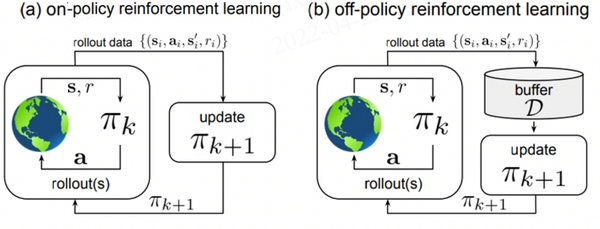
\includegraphics[width=1\linewidth]{figures/on_off_policies.png}
    \caption{Data flow of on-policy vs off-policy}
    \label{fig:on_off_policies}
\end{figure}
Intuitively, we can see their strengths and weaknesses (Tab. \ref{tab:on_off_policies}).
\begin{table}[htb]
    \centering
    \caption{Pros \& cons of on-policy vs off-policy}
    \begin{tabular}{l p{6cm} p{6cm}}
        \toprule
        \textbf{ } & \textbf{On-Policy RL} & \textbf{Off-Policy RL} \\
        \midrule
        \addlinespace
        \textbf{Pros} & Ensures consistency between the improved policy and the data used for learning, leading to stable learning. & Can use experience generated from a different policy, allowing for more flexible data usage and potentially faster learning. \\
        \addlinespace
        \textbf{Cons} & Learning is tied to the policy being executed, which can be less efficient since the agent needs to explore while improving the policy. & learning can be unstable or divergent if buffered policies are too different. \\
        \addlinespace
        \textbf{Use When} & When the policy needs to be improved and evaluated simultaneously. & When leveraging off-policy data, such as using historical data or learning from demonstrations, is advantageous. \\
        \bottomrule
    \end{tabular}
\label{tab:on_off_policies}
\end{table}


\subsection{Model Structure} \label{sec:model_structure}
So far, we have seen how an agent learns from its experience. Specifically, equation \ref{eq:pistar} suggests we can have three distinct implementations. 
\begin{enumerate}
    \item \textbf{Policy-based} methods assume the policy as a function $a = \pi_{\theta}(s)$ whose parameters $\theta$ are recursively estimated using reward feedback. Fair enough, they are often called “an actor”.
    \item \textbf{Value-based} methods calculate the value function (either $V(s)$ or $Q(s, a)$). Then, the agents pick their action by a simple $\max$ operator. Similarly, they can be called “a critic”.
    \item \textbf{Actor-Critic} framework combines them for the best performance when an actor or critic cannot solve the problem alone.
\end{enumerate}
The choice depends on how hard the problem is, the characteristics of the environment, and our computing resources. Table \ref{tab:rl_techniques} compares these three implementations.
\begin{table}[htb]
    \centering
    \caption{Three primary learning methods in RL}
    \label{tab:rl_techniques}
    \begin{tabular}{l p{6cm} p{6cm}}
        \toprule
        \textbf{Method} & \textbf{Advantages} & \textbf{Disadvantages} \\
        \midrule
        Policy-based & Effective in high-dimensional continuous action spaces. Can handle complex policies. & High variance, slow convergence, exploration challenges. \\
        \addlinespace
        Value-based & Efficient for discrete action spaces. It provides a natural way to compare actions. & Struggles with continuous action spaces and sensitive to hyperparameters. \\
        \addlinespace
        Actor-critic & Combines policy optimization and value function estimation. Suitable for continuous action spaces. & Complexity (maintaining both actor and critic networks), absurd hyperparameter tuning. \\
        \bottomrule
    \end{tabular}
\end{table}
At this stage, we have gathered sufficient information to create a \textbf{model-free} agent. Plus, we can enhance our training process by introducing an environment's clone directly to the agent's decision-making process, resulting in a \textbf{model-based} agent (Fig. \ref{fig:model_basedRL}). The choice between these two paradigms is crucial; see more in table \ref{tab:modeled_rl}. With extra information about its environment, an agent converges more rapidly with fewer actions, as it can anticipate future consequences. However, relying on a presumed model may lead to incorrect dynamics in real-world scenarios, limiting the agent's adaptability to varied situations. The accumulated error amplifies when the agent needs to make many predictions ahead, discouraging utilization of model-based in many stochastic contexts \cite{janner2021trust, janner2019mbpo, wang2019benchmarking}. Bansal et al. \cite{bansal2017mbmf} invented a hybrid proposal that uses a Gaussian process to parameterize the system's dynamics and a Bayesian optimizer to search for the optimal policy simultaneously. Although this looks prospective, its complex implementation has not been published.
\begin{figure}[htbp]
    \centering
    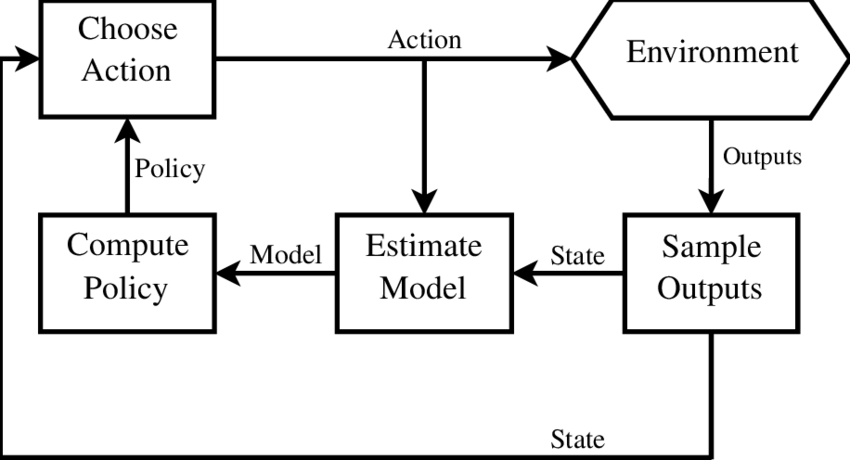
\includegraphics[width=0.75\linewidth]{figures/model_basedRL.png}
    \caption{Model based RL}
    \label{fig:model_basedRL}
\end{figure}

\begin{table}[htbp]
    \centering
    \caption{Model-based vs model-free RL}
    \label{tab:modeled_rl}
    \begin{tabular}{l p{6cm} p{6cm}}
        \toprule
        \textbf{ } & \textbf{Model-based} & \textbf{Model-free} \\
        \midrule
         \textbf{Pros} & Predictable future states and actions without waiting for feedback from the actual environment, making this quicker and more data-efficient & Straightforward, with no need for an explicit model of the environment that usually implies lots of presumptions \\
        \addlinespace
         \textbf{Cons} & Building an accurate environment's model is challenging, and errors in the model may propagate, leading to suboptimal decisions; planning with a learned model may introduce computational overhead & May require more exploration to discover optimal policies, particularly in environments with sparse rewards or deceptive dynamics \\
         \addlinespace
         \textbf{Use when} & Real-time planning is crucial, or the environment's dynamics are stable and predictable & The environment's dynamics are too complex or completely unknown \\
        \bottomrule
    \end{tabular}
\end{table}


\subsection{Interaction with Environment}
Another dimension in categorizing RL types is their interaction with the environment. \textbf{Online} agents learn in real-time while interacting with the environment. It receives feedback after each action and continuously adapts its behavior based on this feedback. They are well-suited for scenarios where the environment's dynamics constantly change, or immediate decision-making is required. However, online learning can be sensitive to noisy or delayed feedback, so the agent must balance exploration and exploitation to learn an optimal policy effectively.

On the other hand, \textbf{offline} agents, aka. "batch RL" or "offline policy evaluation," learn from a fixed dataset of experience samples collected independently of the learning process. This dataset typically consists of trajectories or episodes of interactions between a fixed policy and the environment. Based on this fixed dataset, the agent aims to learn a policy or value function that maximizes the expected return. Offline RL is helpful when collecting new data is expensive, time-consuming, or impractical, such as in healthcare applications or when dealing with sensitive environments. However, this type of interaction poses many challenges, such as sample inefficiency, distributional shift, and handling off-policy data. Both online and offline styles have their respective advantages and challenges, and the choice between them depends on factors such as the availability of real-time feedback, the cost of data collection, and the stability requirements of the learning process.


\subsection{Action and State Types}
The environment solely determines the characters of action and state observation, i.e., \textbf{continuous or discrete}, \textbf{finite or infinite}. For example:
\begin{enumerate}
    \item In a maze-solving game, states are discrete with a finite number of possibilities (position of the agent); actions are the same with either moving up, down, right, or left.
    \item In a chess game, states are discrete and infinitely many; available actions at each state are discrete and finite.
    \item In a self-driving car, states (car position, velocity, disturbances, etc.) and actions (steering wheel position, gas pedal degree, etc.) are continuous values, hence being infinite. 
\end{enumerate}
Example No. 1 is the easiest and fastest to train as it requires the least exploration, whereas examples No. 2 and 3 might take a few days to learn.

Furthermore, actions can be \textbf{stochastic or deterministic}, each with distinct advantages and challenges. Stochastic actions involve selecting an action according to a probability distribution, which allows for exploration of the environment and can help the agent avoid getting stuck in local optima. This approach is instrumental in complex environments where the optimal policy is not understood or multiple equally good ones exist. Conversely, deterministic actions involve selecting the action that maximizes the expected reward based on the current policy. This can lead to more stable and predictable behavior, making evaluation and refinement easier. However, deterministic actions might lead to suboptimal solutions if the agent fails to explore sufficiently and overlooks better alternatives. That is why balancing between exploration and exploitation for both types is crucial for any RL problem. We can achieve this with techniques like epsilon-greedy, additive Gaussian noise for deterministic policy, or softmax action selection \cite{rlbible_multibandit}.


\section{Common RL Algorithms} \label{sec:rlagents}
In this section, I examine some papers that work explicitly on RL for floor heating, HVAC, and thermodynamics control. They are organized by model structure.

\subsection{Value-based}
Let us start with Q-learning \cite{watkins1992qlearning}, the most straightforward scheme in this group. Since its first creation in 1992, many engineers have quickly adopted it and achieved remarkable results \citep{ISSN0360-5442, chen2019gnu, cho2006application, li2015multi}. However, Q-learning depends on a Q-table to map state-action pairs into values, which only works for a discrete, finite set of states and actions (Fig. \ref{fig:qtable}).
\begin{figure}
    \centering
    \begin{subfigure}[t]{0.75\textwidth}
        \centering
        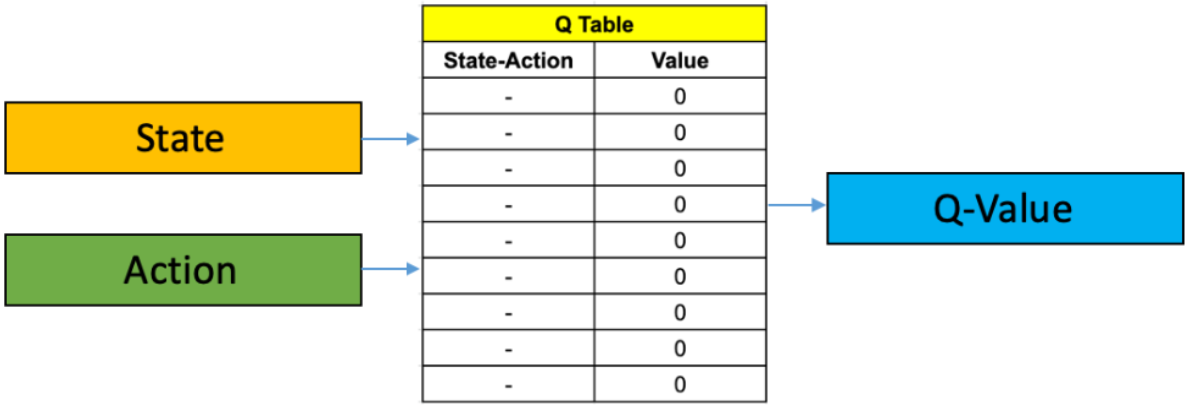
\includegraphics[width=\linewidth]{figures/qtable.png}
        \caption{Q-table in a Q-learning agent}
        \label{fig:qtable}
    \end{subfigure}
    \begin{subfigure}[t]{0.75\textwidth}
        \centering
        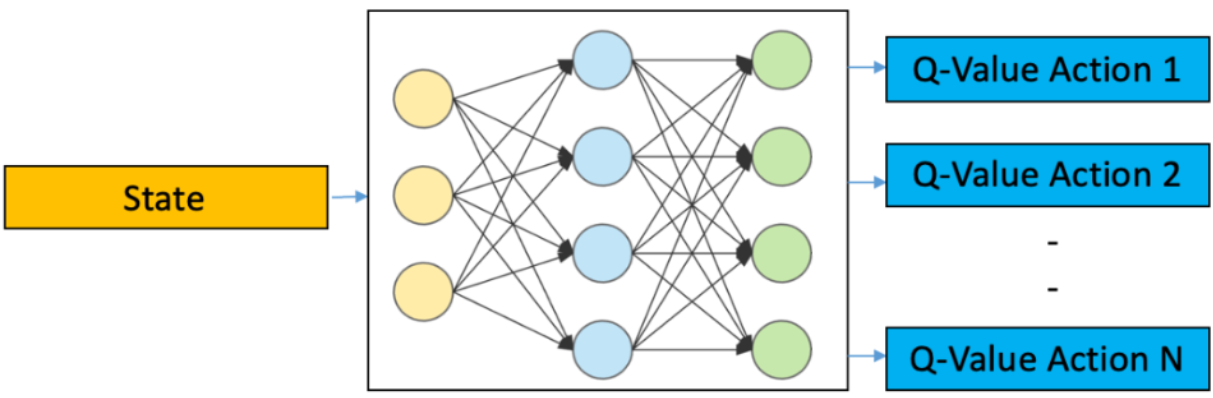
\includegraphics[width=\linewidth]{figures/dqn.png}
        \caption{Neural network as an alternative}
        \label{fig:dqn}
    \end{subfigure}
\caption{Q-learning vs Deep Q-Network}
\end{figure}

To overcome this constraint, in 2013, Mnih et al. \cite{mnih2013playing} invented a Deep Q-network (DQN), a neural-network alternative for the Q-table that can universally estimate a continuous state into action. Wei et al. \cite{wei2017deep} was among the first to adopt DQN in HVAC systems. His early success has led to many adoptions later on \cite{barrett2015autonomous, jia2019advanced}. Most notably, Blad et al. \cite{blad2019control} mainly addressed the problem of slow thermodynamics in HVAC systems, yielding state-of-the-art (SOTA) performance. Junior \cite{junior22} later verified these findings with only five actions:
\begin{itemize}
    \item keep the same duty cycle as in the previous step
    \item increase or decrease $\pm 5$ (\%) from the previous step 
    \item increase or decrease $\pm 2.5$ (\%)
\end{itemize}
In this project, he showed that a DQN could reduce energy consumption by up to 8.8\% with much fewer relay clicks.

As we can see, Q-learning and Deep Q-network are \textbf{model-free, online, off-policy, value-based} agents. As I pointed out in section \ref{sec:model_structure}, an off-policy model might diverge if its past experiences vary too much. SARSA comes in handy by adding a memory buffer, hence the alias “an on-policy Q-learning” \cite{fu2018sarsa}. Still, it was only a proof-of-concept without any noticeable improvement, while the discrete action caveat remains (Fig. \ref{fig:dqn}), hindering an even smoother performance. 

\nomenclature[D]{SOTA}{State-of-the-art, the best performance achieved on a given benchmark.}


\subsection{Policy-based}
A counterpart of Q-learning in continuous-action space is Policy Gradient (PG), introduced by Williams J. \cite{williams1992pg} in 1992. Interestingly, PG agents can work with both action types:
\begin{itemize}
    \item Discrete: the probability of taking each discrete action. The sum of these probabilities across all actions is 1. Thus, the output layer of the actor is often a softmax.
    \item Continuous: the mean and standard deviation of a Gaussian action, hence being called a “stochastic actor.”
\end{itemize}
Such flexibility comes from their underlying REINFORCE, a variation of the Monte Carlo paradigm (Sec. \ref{sec:mdp_solutions}), which can either use the original form (Eq. \ref{eq:montecarlo} with advantage function) or a simplified form with only the discounted future reward (Eq. \ref{eq:future_rwd}). As a result, PGs belong to the Monte Carlo subgroup; they do not learn during an episode but only after it is finished. Although the first form continually updates a V-value function, it does not fully act as a critic; it is not used for bootstrapping, i.e., updating a state's value based on subsequent state estimates. Thus, scientists classify a naive PG as \textbf{model-free, online, on-policy, policy-based}.

Ding et al. \cite{ding2019octopus} was among the first to apply PG for controlling an HVAC system. Yet, their model-free character is too data-hungry, refraining from wide adoption. Later papers proposed model-based alternatives \cite{ding2020mb2c, chen2019gnu, an2024beyondblackboxpolicies} with either a decision tree or a linear regression. Despite being more data efficient, I argue that model-based approaches have too many presumptions, most of which are almost inaccurate or infeasible for real life \cite{gu2016deep, bairblog_modelbasedrl}. Similar to SARSA, PGs are no longer used extensively in the industry. They only serve as examples for educational purposes.

\subsection{Actor-Critic} \label{sec:actor_critic}
So far, we have seen the value-based (critic-only) and policy-based (actor-only) types. Now comes the novel actor-critic (AC) framework. Originally, AC was a standalone algorithm invented by Mnih et al. \cite{mnih2016asynchronous} before being advanced and becoming a whole new RL class. It is a \textbf{model-free, online, on-policy} method that optimizes the policy (actor) directly and simultaneously trains a critic to estimate the expected future reward $G$ (Eq. \ref{eq:future_rwd}). AC can work for both discrete and continuous actions like PG. One of the first authors to use naive AC was Huang et al. \cite{huang2020hvac}. However, there exist some limitations. First, it lacks explicit exploration incentives, often resulting in suboptimal policies. Second, it typically optimizes a stochastic policy, which can be restrictive in low-variance environments. Lastly, being on-policy demands countless amounts of fresh data from trials.

From a cost perspective, Advantage Actor-Critic (A2C) and Asynchronous Advantage Actor-Critic (A3C), two derivations of the naive AC, made training much faster and more accurate by updating the advantage function $\delta_t$ (Eq. \ref{eq:montecarlo}) in multiple CPU threads. Sebastian's thesis \cite{seb23} was one of a few projects that studied HVAC control systems in this direction. Yet, they could not overcome the constraint of being on-policy.

In contrast, the Soft Actor-Critic (SAC) framework of Tuomas et al. \cite{haarnoja2019soft} fully addressed these limitations. It introduces an entropy term to encourage exploration, resulting in more flexible and expressive stochastic policies. SAC is an off-policy algorithm, allowing it to learn from past experiences stored in a replay buffer. By simultaneously learning a value function and a policy, SAC achieves stability and improved sample efficiency. Overall, SAC combines the benefits of stochastic policy optimization, entropy regularization, and off-policy learning to enhance exploration, resulting in many SOTA benchmarks \cite{en14040997, manjavacas2024experimental} in 2020-21. Yet, I am still skeptical of its reliability for being inherently random.

Like AC, Trust Region Policy Optimization (TRPO) is another \textbf{model-free, online, on-policy, stochastic actor} method created by Schulman et al. \cite{schulman2015trust} from Google Deepmind in 2015. Their target was to prevent performance drops by keeping the updated policy within a trust region close to the current policy. In return, TRPO is painfully slow and computationally heavy since it alternates between sampling data through environmental interaction and updating the policy parameters by solving a constrained optimization problem. Consequently, the same authors released a simplified version named Proximal Policy Optimization (PPO) \cite{schulman2017proximal} with fewer hyperparameters, hence a comparable performance with much more efficient training. These papers have shown unbelievable results in various control tasks, from driving a drone to picking up objects with a robot arm. However, their arbitrary nature was proven unstable and cannot enforce exploration within its trust region \cite{wang2020truly}.

Regarding a renovation for SAC, Deep Deterministic Policy Gradient (DDPG) \cite{lillicrap2019ddpg} is one of the most advanced techniques that inherits SAC's strengths to adapt specifically to continuous, deterministic action. Many applications of DDPG to HVAC for large buildings proved its outstanding capability \cite{duyan20multiddpg,fu21mpctd3}. But, it is too prone to hyperparameters. For example, either a too-small (1e-5) or too-large (1e-3) learning rate would stop the agent from learning. This phenomenon is caused by using a deep neural network to calculate the temporal difference in equation \ref{eq:tdq} whose operator $\max$ often overestimates the added noise. As such, Scott et al. \cite{td3} proposed a Twin-Delayed Deep Deterministic (TD3) Policy Gradient agent with three modifications to DDPG that make it way more robust:
\begin{enumerate}
    \item A TD3 agent learns two Q-value functions and uses the minimum value function estimate during policy updates
    \item A TD3 agent updates the policy and targets less frequently than the Q functions
    \item When updating the policy, a TD3 agent adds noise to the target action, which makes the policy less likely to exploit actions with high Q-value estimates.
\end{enumerate}
Unfortunately, TD3 has not been extensively verified on actual HVAC systems, while the original paper showed its superiority in similar control tasks. Some noticeable results \cite{fu21mpctd3,manjavacas2024experimental} are either hybrid methods (with model-based support) or unrealistic computer simulation.

\nomenclature[D]{SAC}{Soft Actor-Critic, an early morphing of the vanilla AC framework}
\nomenclature[D]{A3C}{Asynchronous version of A2C}
\nomenclature[D]{TRPO}{Trust Region Policy Optimization, a model-free, online, on-policy, stochastic-actor RL agent}
\nomenclature[D]{PPO}{Proximal Policy Optimization, a modification of TRPO}
\nomenclature[D]{DDPG}{Deep Deterministic Policy Gradient, a model-free, online, off-policy, deterministic-actor RL agent}
\nomenclature[D]{TD3}{Twin-Delayed Deep Deterministic Policy Gradient, a modification of DDPG}


\section{Summary of Literature Review}
Table \ref{tab:rlagents} summarizes all algorithms mentioned above (Sec. \ref{sec:rlagents}). 
\begin{table}[htb]
    \centering
    \caption{RL Algorithms Categories}
    \begin{tabular}{l p{4cm} p{4cm} p{4cm}}
    \hline
    \textbf{Value Type} & \textbf{No Actor} & \textbf{Stochastic Actor} & \textbf{Deterministic Actor} \\ \hline
    \textbf{V-Value} &  & Policy Gradient, original Actor-Critic, PPO, TRPO &  \\ \hline
    \textbf{Q-Value} & Q-Learning, SARSA, DQN &  & SAC, DDPG, TD3 \\ \hline
    \end{tabular}
    \label{tab:rlagents}
\end{table}
Despite many proofs of their capability, applying RL to a realistic dynamical system remains challenging because of the need for accurate system modeling, vast data availability, stability, and safety concerns \cite{sierla2022review, paleyes2022challenges}. These problems still hold in OJ's floor heating (FHEL) context.
\begin{itemize}
    \item Safety concern, e.g., a wooden floor must not be heated up to 35\degree C, whereas a concrete floor cannot drop below 5\degree C. Also, a decision must be consistent and predictable. Thus, a deterministic actor is more suitable than a stochastic one.
    \item States and actions are naturally continuous. Hence, a tabular policy or discrete actors like Q-learning and DQN are unsuitable.
    \item Limited computing resources but a vast amount of time. Hence, there is no problem with a mid-size deep neural network or model-free agents.
    \item Ease of development and fine-tuning. TRPO and DDPG are eliminated as they are too sensitive to hyperparameters, even for a random seed generator, making the research more of an endless trial-and-error.
    \item A unified development toolbox that supports RL training and control system debugging. Thus, I use MATLAB/Simulink.
    \item Expand the horizon of undiscovered directions
\end{itemize}
After carefully considering those aspects, I decide to use a Twin-Delayed Deep Deterministic Policy Gradient (TD3) as my primary controller.

\end{document}